\documentclass[ 12pt ]{article}
\usepackage{amsmath, amsthm, amssymb, csquotes, enumitem, graphicx, listings, mathrsfs}
\usepackage[margin=0.5in]{geometry}
\graphicspath{ ./ }

\begin{document}

\noindent Landon Fox \\
\noindent Math 440 \\
\noindent April 24, 2021

\begin{center}
	\Large Problem Set 5
\end{center}

\begin{enumerate}
	% problem 1
	\item[\textbf{1.}]
		\begin{enumerate}
			\item[\textbf{a.}] Show that if $A \subseteq \mathbb{R}$ is compact, then $\sup A \in A$ and $\inf A \in A$.
			\item[\textbf{b.}] Prove the following generalization of the Extreme Value Theorem.
				\begin{displayquote}
					Let $X$ be a compact topological space and $f : X \to \mathbb{R}$ a continuous function. Then there exists an $x \in X$ such that $|y| \leq |f(x)|$ for all $y \in
					f(X)$.
				\end{displayquote}
		\end{enumerate}

		\begin{proof} $ $
			\begin{enumerate}
				\item[\textbf{a.}] Suppose $A \subseteq \mathbb{R}$ is compact. Then by Heine-Borel, we know that $A$ is both bounded and closed. Moreover, there exists values $a, b \in
					\mathbb{R}$ such that $A \subseteq [a, b]$ and so $$\inf A \leq \sup A \in [a, b] \subseteq \mathbb{R}$$ as a result of its definition. From analysis, we know that we
					can find an element of $A$ arbitrarily close to $\sup A$ ($\inf A$, respectively). Consider a sequence $\{ x_k \}_{k \in \mathbb{N}}$ with the property $$x_k \in A
					\cap B_{1/k}(\sup A)\;\;\; (A \cap B_{1/k}(\inf A),\; \mathrm{respectively}).$$ Clearly, we can see that $\lim_{k \to \infty} x_k = \sup A$ ($\inf A$) is a limit
					point of $A$ and so $\sup A \in A$ ($\inf A \in A$) because $A$ is closed.

				\item[\textbf{b.}] Let $X$ be a compact topological space and $f : X \to \mathbb{R}$ a continuous function. By Theorem 23.6 it follows that $f(X) \subseteq \mathbb{R}$
					is compact. Then by \textbf{1a} there exists an $x \in X$ such that $f(x) = \sup f(X)$ ($\inf f(X)$, respectively) and so $$|y| \leq \max\{ |\inf f(X)|,\,
					|\sup f(X)| \}$$ holds for all $y \in f(X)$, proving the assertion.
			\end{enumerate}
		\end{proof}


	% problem 2
	\item[\textbf{2.}]
		\begin{enumerate}
			\item[\textbf{a.}] Show that if $X$ is compact, then the projection $p_Y : X \times Y \to Y$ is a closed map.
			\item[\textbf{b.}] Give an example of spaces $X$ and $Y$ such that the projection $p_Y$ is not a closed map.
		\end{enumerate}

		\begin{proof} $ $
			\begin{enumerate}
				\item[\textbf{a.}] Suppose $X$ and $Y$ are topological spaces with $X$ compact. We know that the projection $p_Y$ is a continuous function; therefore, it suffices to
					show that $p_Y$ is closed. Consider a closed subset $Z \subseteq X \times Y$ and its projection $p_Y(Z) \subseteq Y$. Further, we may assume there exists a $y \in Y$
					such that $y \notin p_Y(Z)$. Then it follows that $X \times \{ y \} \subseteq X \times Y$ and $Z$ are disjoint. Since $X \times Y \setminus Z$ is an open subset, we
					may consider the collection of open subsets that comprise the subset. Let $\mathcal{W}$ denote a subcollection of such open subsets that have a nonempty intersection
					with $X \times \{ y \}$. Then by the Tube Lemma there exists a finite cover $\mathcal{U} = \{ U_i \}_{1 \leq i \leq n}$ of $X$ and an open subset $V \subseteq Y$
					with $y \in V$, such that for all $1 \leq i \leq n$ there exists an open set $W \in \mathcal{W}$ that contains the product $U_i \times V \subseteq X \times Y$.
					Observe that $V$ and $p_Y(Z)$ are disjoint; indeed, if $v \in V$ and $(x, v) \in Z$, then there would exist an open set $U_i$ containing $x$ and an associated $W \in
					\mathcal{W}$, however $$(x, v) \in U_i \times V \subseteq W \subseteq X \times Y \setminus Z$$ is a contradiction. Hence, there exists an open neighborhood $V$ of
					$y$ disjoint to $p_Y(Z)$ illustrating that $p_Y(Z)$ is closed as desired.

				\item[\textbf{b.}] Let $X = Y = \mathbb{R}$. We have shown previously that a plot $\Gamma_f \subseteq \mathbb{R}^2$ is closed for a continuous function $f : \mathbb{R}
					\to \mathbb{R}$. Then $\Gamma_f \subseteq X \times Y$ is a closed subset provided a function $f : X \to Y$ defined as $f(x) = e^x$. However, observe that $p_Y(
					\Gamma_f) = (0, \infty) \subseteq Y$ is open in $Y$.
			\end{enumerate}
		\end{proof}


	% problem 3
	\item[\textbf{3.}] Let $X$ and $Y$ be topological spaces with $Y$ compact Hausdorff. Further, let $f : X \to Y$ be a function and $\Gamma_f \subseteq X \times Y$ its plot. Show that
		$f$ is continuous if and only if $\Gamma_f$ is closed in $X \times Y$.

		\begin{proof}
			Suppose $X$ and $Y$ are topological spaces with $Y$ compact Hausdorff. Additionally, let $f : X \to Y$ be a function and $\Gamma_f \subseteq X \times Y$ its plot. First,
			suppose $f$ is continuous. Consider a point $(x, y) \notin \Gamma_f$, that is $y \neq f(x)$. Due to the Hausdorffness of $Y$, there exists disjoint open subsets $U, V
			\subseteq Y$ containing $f(x)$ and $y$, respectively. Observe that $$(x, y) \in f^{-1}(U) \times V \subseteq (X \times Y) \setminus \Gamma_f;$$ indeed, if $(u, v) \in
			f^{-1}(U) \times V$, then $f(u) \in U$ which is disjoint to $V$ implying that $f(u) \neq v$. Now, we can see that $f^{-1}(U)$ is open since $f$ is continuous and so
			$f^{-1}(U) \times V$ is open in $X \times Y$. Thus, $\Gamma_f$ is closed since $f^{-1}(U) \times V$ is an open neighborhood of $(x, y)$. \\

			Conversely, let us now suppose $\Gamma_f$ is closed. Let $V \subseteq Y$ be an arbitrary open subset containing a point $f(x)$. Then it follows that $$\Gamma_f \cap
			\left ( (X \times Y) \setminus (X \times V) \right ) = \Gamma_f \cap \left ( X \times (Y \setminus V) \right ) \subseteq X \times Y$$ is closed. Additionally, it holds
			that $$A := p_X \left ( \Gamma_f \cap \left ( X \times (Y \setminus V) \right ) \right ) \subseteq X$$ is closed via \textbf{2a}. Notice that $A$ represents the set of
			all points of $X$ that do not have an image in $V$ under $f$. Thus, the image of the open subset $X \setminus A$ is contained in $V$, that is, $$f(x) \in f(X \setminus A)
			\subseteq V$$ and so $f$ is continuous by definition.
			\begin{center}
				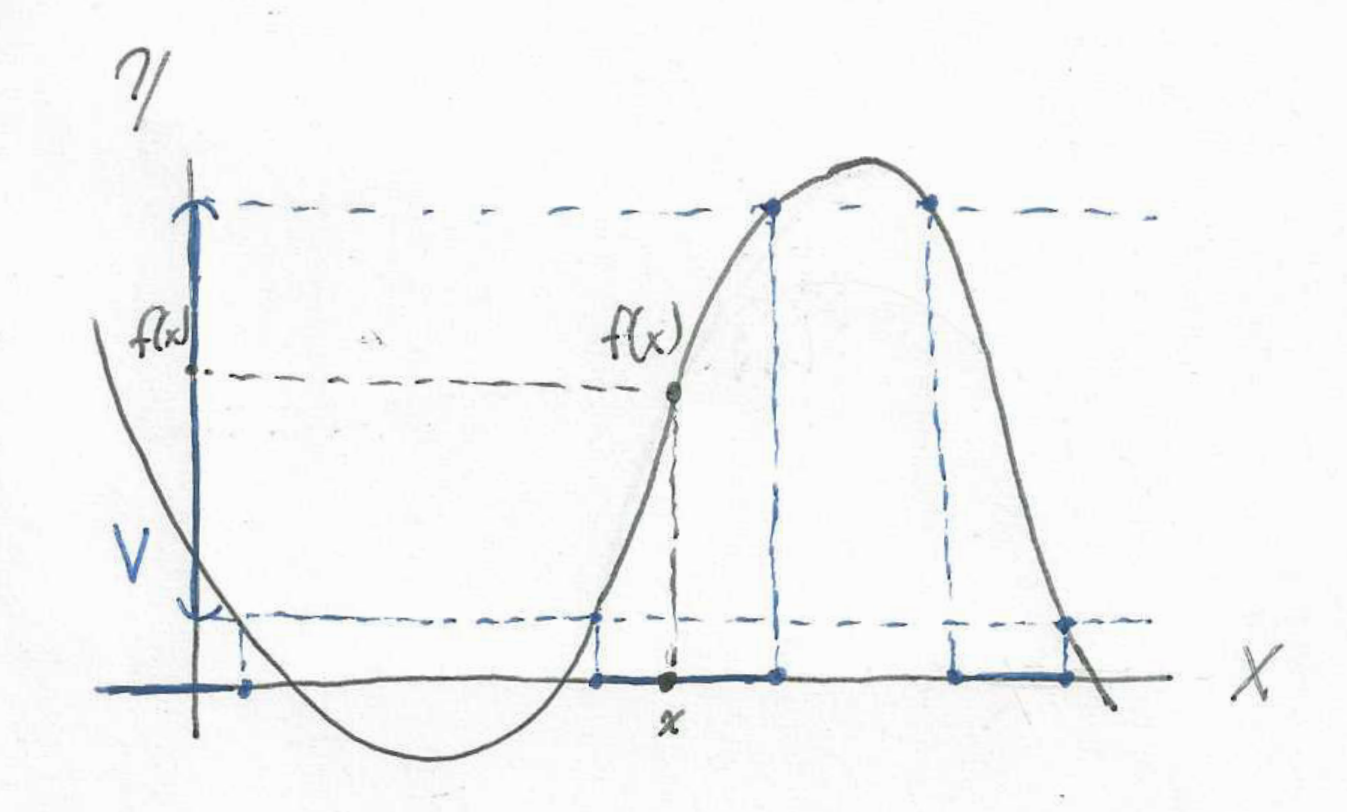
\includegraphics[scale=0.5]{Capture}
			\end{center}
		\end{proof}


	% problem 4
	\item[\textbf{4.}] Let $X$ be a topological space and $S_n$ the symmetric group. Let $S_n$ act on $X^n$ via $T_\sigma : X^n \to X^n$ defined as $$T_\sigma(x_1, x_2, \hdots, x_n)
		= (x_{\sigma(1)}, x_{\sigma(2)}, \hdots, x_{\sigma(n)})$$ for all $\sigma \in S_n$. Show that $T_\sigma$ is a homeomorphism for all $\sigma \in S_n$.

		\begin{proof}
			Suppose $X$ is a topological space and $T_\sigma : X^n \to X^n$ is a group action with $S_n$ acting on $X_n$ as defined above. For an arbitrary permutation $\sigma \in S_n$,
			observe that $$T_\sigma \circ T_{\sigma^{-1}} = T_\mathrm{id} = \mathrm{id} : X^n \to X^n$$ as well as $$T_{\sigma^{-1}} \circ T_\sigma = T_\mathrm{id} = \mathrm{id} : X^n
			\to X^n$$ and so $T_\sigma$ is invertible by definition with $T_{\sigma^{-1}}$ as its inverse. \\

			In regard to continuity, it suffices to show that $T_\sigma$ is continuous for an arbitrary $\sigma \in S_n$ since its inverse, $T_\sigma^{-1} = T_{\sigma^{-1}}$, utilizes
			another permutation $\sigma^{-1}$. Consider an open subset $U \subseteq X^n$ in $\mathrm{cod}\, T_\sigma$ and a collection of basis elements $$\mathcal{U} = \left \{ U_{i_1}
			\times U_{i_2} \times \hdots \times U_{i_n} \right \}_{i_k \in \mathcal{I}}$$ with $$\bigcup_{i_k \in \mathcal{I}} U_{i_1} \times U_{i_2} \times \hdots \times U_{i_n} = U$$
			where each $U_{i_k} \subseteq X$ is open. Then it follows that $$T_\sigma^{-1}(U) = T_{\sigma^{-1}}(U) = \bigcup_{i_k \in \mathcal{I}} T_{\sigma^{-1}} \left ( U_{i_1} \times
			U_{i_2} \times \hdots \times U_{i_n} \right ) = \bigcup_{i_k \in \mathcal{I}} U_{i_{\sigma^{-1}(1)}} \times U_{i_{\sigma^{-1}(2)}} \times \hdots \times U_{i_{\sigma^{-1}
			(n)}}$$ is open in $\mathrm{dom}\, T_\sigma$. Hence, $T_\sigma$ is a homeomorphism.
		\end{proof}


	% problem 5
	\item[\textbf{5.}] Prove that if $X$ is an infinite set, then the cofinite topology $(X, \mathcal{T}_\mathrm{cof})$ is a connected space.

		\begin{proof}
			Let $X$ be an infinite set. Consider a nonempty open proper subset $U \subset X$ in $(X, \mathcal{T}_\mathrm{cof})$. Then $X \setminus U$ is a finite set by definition.
			Observe that $U$ cannot be finite since $$|U| = |X| - |X \setminus U|$$ is infinite. Thus, $U$ cannot be closed and so $(X, \mathcal{T}_\mathrm{cof})$ is connected by
			Proposition 31.2.
		\end{proof}


	% problem 6
	\item[\textbf{6.}] Show that for any set $X$, the discrete topology $(X, \mathcal{T}_\mathrm{disc})$ is totally disconnected. Additionally, show that the converse does not hold.

		\begin{proof}
			Let $X$ be a set and consider the discrete topology $(X, \mathcal{T}_\mathrm{disc})$. It is obvious that any singleton of any set under any topology is a connected component,
			so then we will turn to subspaces with cardinality exceeding 1. Suppose $A \subseteq X$ is a subspace of $(X, \mathcal{T}_\mathrm{disc})$ with $|A| \geq 2$. Then by
			definition, any bipartition of $A$ provides disjoint closed subsets covering $A$ implying disconnectedness via Proposition 31.2. Hence, $(X, \mathcal{T}_\mathrm{disc})$ is
			totally disconnected by definition. \\

			In regard to the converse of the assertion, the rationals equipped with the Euclidean subspace topology provides a counterexample. Clearly, we can see that $(\mathbb{Q},
			\mathcal{T}_\mathrm{Euc}) \neq (\mathbb{Q}, \mathcal{T}_\mathrm{disc})$ (the singleton $\{ q \} \notin \mathcal{T}_\mathrm{Euc}$ for all $q \in \mathbb{Q}$, for instance).
			Now, consider any subspace $A \subseteq \mathbb{Q}$ with $|A| \geq 2$. It follows that for any $a < b \in A$ there exists an irrational $x \in \mathbb{R} \setminus
			\mathbb{Q}$ such that $a < x < b$. Therefore, $[a, b] \nsubseteq A$ and so $A$ is not connected by Theorem 32.1.
		\end{proof}


	% problem 7
	\item[\textbf{7.}] Demonstrate that $\mathbb{R}_\ell$ is disconnected.

		\begin{proof}
			Let $b \in \mathbb{R}$. Observe that the following open sets $$\left ( \bigcup_{a < b} [a, b) \right ) \bigcup \left ( \bigcup_{b < c} [b, c) \right ) = \mathbb{R}$$
			partition $\mathbb{R}_\ell$ and so $\mathbb{R}_\ell$ is disconnected by definition.
		\end{proof}


	% problem 8
	\item[\textbf{8.}] Show that the connected components of $\mathbb{Q} \subseteq \mathbb{R}$ are not open.

		\begin{proof}
			From the counterexample in \textbf{6}, we know that $\mathbb{Q} \subseteq \mathbb{R}$ is a totally disconnected space illustrating that only singletons are connected
			which we know to be nonopen in both $\mathbb{Q}$ and $\mathbb{R}$.
		\end{proof}

	% problem 640, 2
	\item[\textbf{640, 2.}]
		\begin{enumerate}
			\item[\textbf{a.}] Show that $\mathrm{GL}_n(\mathbb{C})$ is dense in $\mathrm{Mat}_n(\mathbb{C})$.
			\item[\textbf{b.}] Let $t \in \mathbb{C}$ and $A \in \mathrm{Mat}_n(\mathbb{C})$. Verify that the following functions
				\begin{center}
				\begin{tabular}{ll}
					$p_1 : \mathrm{Mat}_n(\mathbb{C}) \to \mathbb{C}$ & $p_2 : \mathrm{Mat}_n(\mathbb{C}) \to \mathbb{C}$ \\
					$p_1(M) = \det( AM - tI )$ & $p_2(M) = \det( MA - tI )$
				\end{tabular}
				\end{center}
				are continuous.
			\item[\textbf{c.}] Prove that for all $A, B \in \mathrm{Mat}_n(\mathbb{C})$, the spectrum of $AB$ and $BA$ are equal.
		\end{enumerate}

		\begin{proof} $ $
			\begin{enumerate}
				\item[\textbf{a.}] Let $A \in \mathrm{Mat}_n(\mathbb{C})$, $B \in \mathrm{GL}_n(\mathbb{C})$, and consider the polynomial $q : \mathrm{Mat}_n(\mathbb{C}) \to \mathbb{C}$
					defined as $$q(t) = \det( (1 - t)A + tB ) \in \mathbb{C}[t]$$. Observe that $q \neq 0$, that is, the zero polynomial since $q(1) = \det B \neq 0$. Furthermore, since
					$\deg q \leq n$, it must hold that $q$ has a finite number of roots and so the convex combination $(1 - t)A + tB$ has a finite number of singular matrices. Therefore,
					the aforementioned line segment must have a nonsingular matrix contained within the open ball $B_\epsilon(A) \subseteq \mathrm{Mat}_n(\mathbb{C})$ for all $\epsilon >
					0$, otherwise implying there is an infinite number of roots of $q$ covering the line segment within the open ball. Hence, every open subset of $\mathrm{Mat}_n(
					\mathbb{C})$ has a nonempty intersection with $\mathrm{GL}_n(\mathbb{C})$, proving the assertion.

				\item[\textbf{b.}] \textit{The following justification is informal.} Suppose $t \in \mathbb{C}$, $A \in \mathrm{Mat}_n(\mathbb{C})$, and $p_1, p_2 : \mathrm{Mat}_n(
					\mathbb{C}) \to \mathbb{C}$ are defined as above. Observe that  $\mathrm{Mat}_n(\mathbb{C})$ can be viewed as a collection of vectors over the complex field,
					$\mathbb{C}^{n^2}$. Then matrix multiplication and addition can viewed as vector operations with polynomials as the entries of the resulting vector which
					we know to be continuous from analysis. Then the determinant we know to be a polynomial with respect to matrix entries and so it is a continuous map. Therefore,
					it follows that both $p_1$ and $p_2$ are the composition of continuous functions, illustrating that they are also continuous maps.

				\item[\textbf{c.}] Consider the maps $p_1, p_2 : \mathrm{Mat}_n(\mathbb{C}) \to \mathbb{C}$ as defined above. Let $M \in \mathrm{GL}_n(\mathbb{C})$ and observe that
					\begin{align*}
						p_1(M) &= \det( AM - tI ) \\
						&= \det( M^{-1}MAM - tM^{-1}M ) \\
						&= \det M^{-1} \det( MA - tI ) \det M \\
						&= \det( MA - tI ) \\
						p_1(M) &= p_2(M).
					\end{align*}
					Furthermore, $p_1 = p_2$ on $\mathrm{Mat}_n(\mathbb{C})$ via Corollary 29.5 since $\mathrm{GL}_n(\mathbb{C})$ is dense. Thus, the characteristic polynomial of $AM$
					is equal to $MA$ and so its roots, its eigenvalues, must also.
			\end{enumerate}
		\end{proof}


\end{enumerate}

\end{document}
